\documentclass[a4paper]{article}

\usepackage{times}
\usepackage{tikz}
\usepackage[margin=0cm]{geometry}
\usepackage{graphicx}
\usepackage{anyfontsize}
\usepackage{fancyhdr}
\usepackage{indentfirst}
\usepackage{amsmath}
\usepackage[spanish]{babel}
\usepackage[utf8]{inputenc}
\usepackage{titlesec}
\usepackage{enumitem}
\usepackage{caption}
\usepackage{booktabs}

\author{}
\date{}
\title{}

\begin{document}
\thispagestyle{empty}

\newcommand{\saltoPag}{\newpage \noindent \thispagestyle{fancy}}

\begin{tikzpicture}[remember picture, overlay]
    \pgftransformshift{\pgfpoint{0cm}{0cm}}
    \draw [line width=2pt](1cm,-1cm) -- (1cm,-27.7cm) -- (14cm, -27.7cm) -- (14cm, -1cm) -- (1cm, -1cm);
    \draw[line width=2pt] (15cm, -27.7cm) -- (19cm,-27.7cm) -- (19cm, -1cm) -- (15cm, -1cm) --  (15cm, -27.7cm);
    \node [line width=2pt] at (17cm, -3.5cm) {
\includegraphics[width=3cm]{../imagenes/utn.png}};
		\node [line width=2pt] at (7.5cm, -7.5cm) {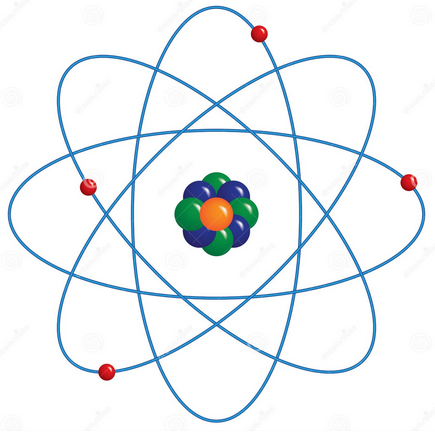
\includegraphics[width=6cm]{../imagenes/fotoAtomo.png}};
    \node at (17cm, -7cm) {\scalebox{5}{\textbf{U}}};
    \node at (17cm, -9cm) {\scalebox{5}{\textbf{T}}};
    \node at (17cm, -11cm) {\scalebox{5}{\textbf{N}}};
    \node at (17cm, -14cm) {\scalebox{5}{\textbf{F}}};
    \node at (17cm, -16cm) {\scalebox{5}{\textbf{R}}};
    \node at (17cm, -18cm) {\scalebox{5}{\textbf{C}}};
    \node at (7.5cm, -13cm) {\scalebox{2.5}{\textbf{Modelo atómico}}};

    \node at (7.5cm, -22cm) {
        \begin{minipage}[c]{12cm}
            \begin{itemize}
                \raggedright
                \vspace{1.5cm}
                \item \fontsize{12}{12}\selectfont \textbf{Autores:} \vspace {1mm} \fontsize{11}{12}\selectfont \\
                    \begin{itemize}
                        \item \hspace{2mm} Valentino Rao - Leg. 402308 \\
                        \item \hspace{2mm} Ignacio Ismael Perea - Leg. 406265 \\
                        \item \hspace{2mm} Manuel Leon Parfait - Leg. 406599 \\ 
                        \item \hspace{2mm} Gonzalo Filsinger - Leg. 400460 \\ 
                        \item \hspace{2mm} Agustín Coronel - Leg. 402010 \\
                        \item \hspace{2mm} Santiago Pannunzio - Leg. 402350 \\
                        \item \hspace{2mm} Marcos Raúl Gatica - Leg. 402006 \\
                    \end{itemize}

                \item \fontsize{12}{12}\selectfont \textbf{Curso:} 2R1. \\
                \item \fontsize{12}{12}\selectfont \textbf{Asignatura:} Física electrónica. \\
                \item \fontsize{12}{12}\selectfont \textbf{Institución:} Universidad Tecnológica Nacional - Facultad Regional de Córdoba \\

            \end{itemize}
        \end{minipage}};

\end{tikzpicture}

\renewcommand{\normalsize}{\fontsize{12}{18}\selectfont}
\newgeometry{margin=2.54cm} %Quiero dejar esto cercano a las normas APA
\fancyhf{}
\renewcommand{\headrulewidth}{0pt}
\renewcommand{\footrulewidth}{0.4pt}
\fancyfoot[R]{[Rao V. - Parfait M. - Filsinger G. - Perea I. - Coronel A - Pannunzio S. - Gatica M.] [\textbf{pág. \thepage}]}
\setlength{\footskip}{1.5cm}
\newpage
\thispagestyle{empty}
\text{}

\titleformat{\section} {\fontsize{12}{12}\bfseries}{\thesection.}{0.5em}{\underline}

\newpage
\newpage

\thispagestyle{empty}
\setcounter{page}{0}
\tableofcontents

\saltoPag
\twocolumn
\flushbottom
\section{INTRODUCCIÓN}

    \indent El siguiente informe busca detallar las prácticas de laboratorio para determinar:

    \begin{itemize}
        \item El valor de la mayor longitud de onda de la serie de Paschen.
        \item La longitud de onda de la línea espectral correspondiente a la transición del hidrógeno de estado n = 6 $\rightarrow$ 3.
        \item Longitud de onda de un fotón emitido por un átomo de hidrógeno al pasar de estado 10 al fundamental.
        \item Energía para extraer un electrón del átomo de hidrógeno en el estado n = 2.
        \item Diferencia de potencial necesaria para acelerar los electrones para que emita la primera línea de la serie de Balmer.
    \end{itemize}

\section{FUNDAMENTOS TEÓRICOS}
    \subsection{Modelo atómico de Thomson}
        \indent El modelo consiste en una masa de carga positiva sobre el cual quedan inmersas cargas negativas [ver figura a continuación]. Las demostraciones que fundamentaban este modelo del átomo no eran del todo adecuados debido al uso de los instrumentos de medición que se usaba. 

        \begin{figure}[h!]
            \centering
            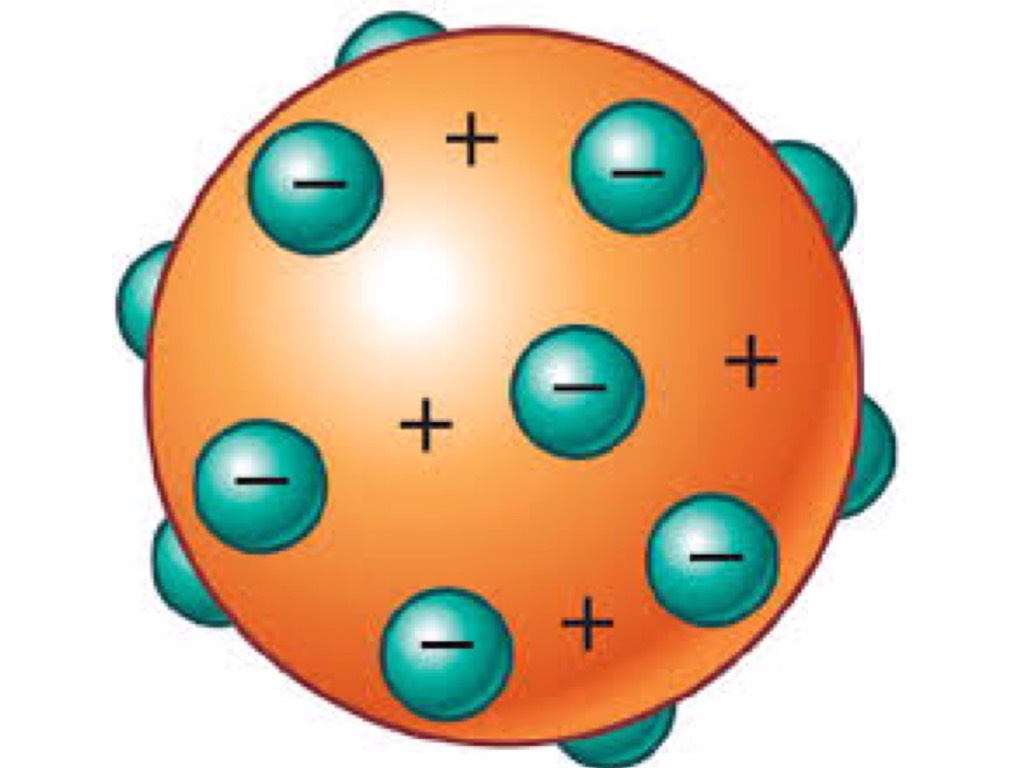
\includegraphics[width=4.5cm]{../imagenes/modeloAtomicoThomson.jpeg}
        \end{figure}

    \subsection{La excitación atómica}
        \indent Se sabe de dos mecanismos fundamentales capaces de excitar a un átomo:

        \renewcommand{\theenumi}{\roman{enumi}}
        \begin{enumerate}
            \item Provocando una interacción del átomo con otra partícula de tal forma que parte de la energía cinética sea absorbida por el átomo (como un choque o que un electrón pase cerca del núcleo atómico).
            \item Cuando un átomo recibe luz en cantidad suficiente para excitarlo.
        \end{enumerate}

        \indent Esto se asocia a darle energía de manera externa al átomo para que uno de sus electrones salte a un nivel de energía más alto (estado excitado). En ese punto, el átomo se vuelve inestable y buscará liberar la energía absorbida (haciéndolo en forma de fotones) para regresar a su estado más estable.
        \indent El o los fotones emitidos producen una línea espectral característica de la energía emitida (base de espectros de emisión).

    \subsection{Espectros atómicos}
        \indent Consiste en el análisis de la longitud de onda de una fuente luminosa. Hay cuatro tipos de clases de espectros:
        \begin{enumerate}
            \item Continuos de emisión.
            \item De líneas de emisión.
            \item Continuos de absorción.
            \item De líneas de absorción.
        \end{enumerate}

        \textbf{I - Continuos de emisión} \\
            \indent Es aquel que ocurre en sólidos a altas temperaturas, como un filamento de tungsteno o wolframio de una lámpara eléctrica.

            \begin{figure}[h!]
                \centering
                
\includegraphics[width=4.5cm]{../imagenes/espectroContinuoDeEmision.png}
            \end{figure}

        \textbf{II - De líneas de emisión} \\
            \indent Se produce por descargas eléctricas en vapor de gas a altas temperaturas.
            \indent Los espectros de emisión se caracterizan por tener líneas claras sobre un fondo oscuro.

            \begin{figure}[h!]
                \centering
                
\includegraphics[width=4.5cm]{../imagenes/espectroLineasDeEmision.png}
            \end{figure}

        \textbf{III - Continuos de absorción}
            \indent Ocurre al hacer pasar un espectro continuo de emisión a través de un material de estado líquido o sólido. Se puede ver una franja con colores faltantes, aquellos que fueron absorbidos por el material en cuestión.

            \begin{figure}[h!]
                \centering
                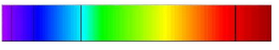
\includegraphics[width=4.5cm]{../imagenes/espectroContinuoDeAbsorcion.png}
            \end{figure}

        \textbf{IV - De líneas de absorción}
            \indent Ocurre cuando la luz pasa por un gas o vapor, el cual absorve algunas de las energías incidentes.

    \subsection{Series espectrales}

        \indent Son un conjunto matemático que determinan el valor de las longitudes de onda presentes en un espectro atómico.

        \textbf{Series espectrales del hidrógeno} \\
            Antes de la formulación de un modelo atómico robusto, los científicos determinaron experimentalmente un conjunto de series espectrales: \\

            \textit{Nota: para todos los casos, R es la constante de Raydberg y es igual a} $1,097 . 10^7 \frac{1}{m}$ \\

            \saltoPag

            \begin{itemize}
                \item \textbf{Serie de Lyman:} funciona para la emisión ultra violeta del hidrógeno, o sea, a altas frecuencias. 
                    \begin{center}
                        $\frac {1}{\lambda} = R(1 - {\frac{1}{n^2}})$ \hspace{2mm} $[n = 2,3,4,...]$
                    \end{center}

                \item \textbf{Serie de Balmer:} funciona para la emisión en el espectro visible.
                    \begin{center}
                        $\frac {1}{\lambda} = R({\frac{1}{2^2}} - {\frac{1}{n^2}})$ \hspace{2mm} $[n = 3,4,5,...]$
                    \end{center}

                \item \textbf{Serie de Paschem:} funciona para la emisión ultra violeta del hidrógeno a altas frecuencias.
                    \begin{center}
                        $\frac {1}{\lambda} = R({\frac{1}{3^2}} - {\frac{1}{n^2}})$ \hspace{2mm} $[n = 4,5,6,...]$
                    \end{center}

                \item \textbf{Serie de Brackett:} funciona para la emisión infrarroja, en bajas frecuencias.
                    \begin{center}
                        $\frac {1}{\lambda} = R({\frac{1}{4^2}} - {\frac{1}{n^2}})$ \hspace{2mm} $[n = 5,6,7,...]$
                    \end{center}

                \item \textbf{Serie de Pfund:} funciona para la emisión infrarroja.
                    \begin{center}
                        $\frac {1}{\lambda} = R({\frac{1}{5^2}} - {\frac{1}{n^2}})$ \hspace{2mm} $[n = 6,7,8,...]$
                    \end{center}
            \end{itemize}
        
\section{Experiencia de laboratorio}

\end{document}
